\section{Resultados}
\label{sec:resultados}

\subsection{Resultados del proyecto}

En esta sección se van a mostrar algunos ejemplos de las predicciones obtenidas con los modelos entrenados con el conjunto de datos que mejores resultados ha obtenido, es decir, con los modelos entrenados con el juego de datos denominado como \textit{filtro 100x40}. Este juego de datos está compuesto por imágenes con baches que como mínimo tienen unas dimensiones de 100x40 píxeles.

\begin{figure}[H]
	\centering
	\begin{subfigure}[h]{0.45\linewidth}
		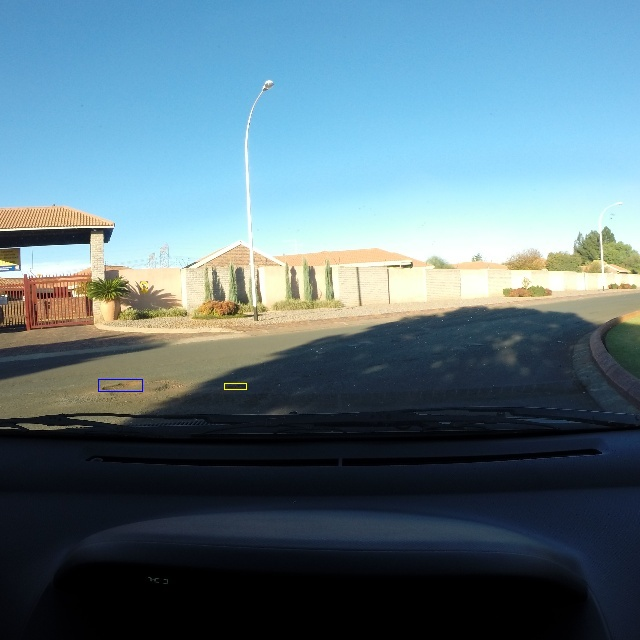
\includegraphics[width=\linewidth]{images/results_a_gt.jpg}
		\caption{Baches a detectar}
	\end{subfigure}
	\begin{subfigure}[h]{0.45\linewidth}
		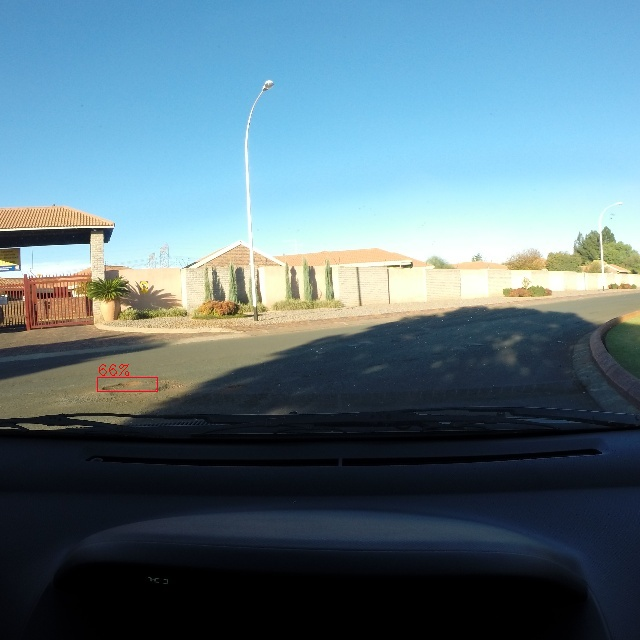
\includegraphics[width=\linewidth]{images/results_a_yolo_v3_256.jpg}
		\caption{YOLO V3 tamaño 256x256}
	\end{subfigure}
	\begin{subfigure}[h]{0.45\linewidth}
		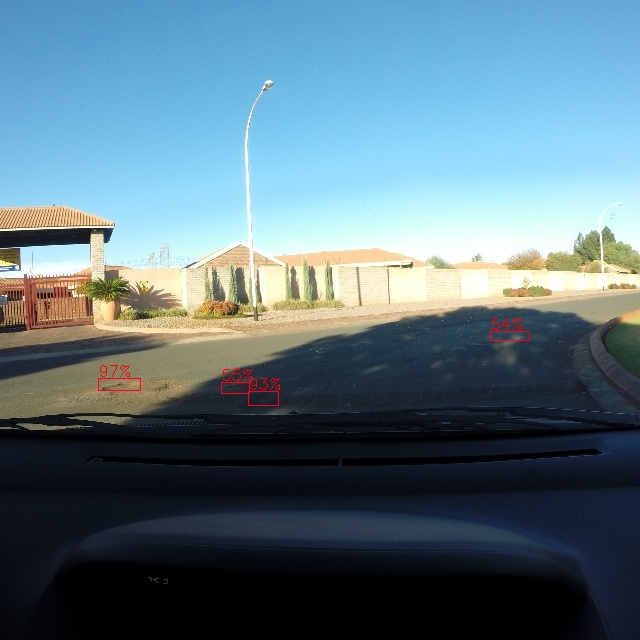
\includegraphics[width=\linewidth]{images/results_a_yolo_v3_416.jpg}
		\caption{YOLO V3 tamaño 416x416}
	\end{subfigure}
	\begin{subfigure}[h]{0.45\linewidth}
		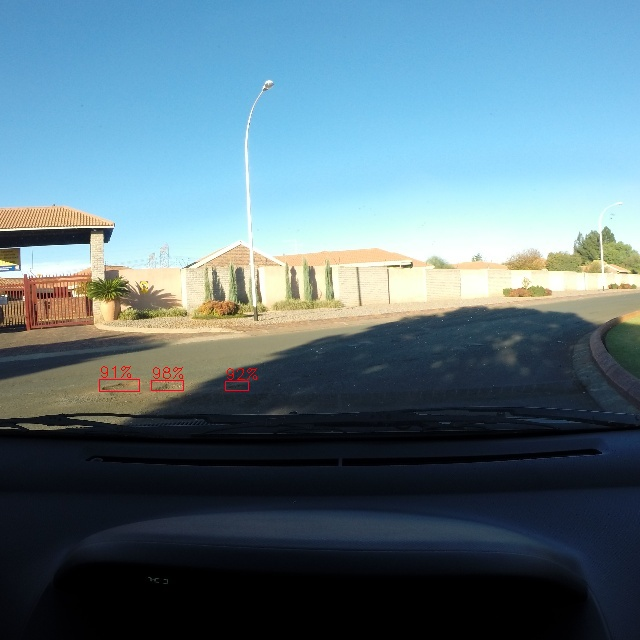
\includegraphics[width=\linewidth]{images/results_a_yolo_v3_640.jpg}
		\caption{YOLO V3 tamaño 640x640}
	\end{subfigure}
	\caption{Ejemplo de predicción con modelos YOLO V3 de distintos tamaños. Arriba a la izquierda, la imagen con los baches a detectar en azul y en amarillo los baches que fueron descartados por el filtro. En el resto de las imágenes se pueden ver las predicciones realizadas en rojo.}
	\label{fig:resultsav3}
\end{figure}

En la figura \ref{fig:resultsav3} se muestran las predicciones realizadas por los modelos YOLO V3. Se trata de una imagen en la que originalmente se han etiquetado 2 baches, uno de los cuales se ha descartado por ser demasiado pequeño. Se puede observar que existe un defecto en el etiquetado, ya que entre los dos baches etiquetados existe un tercer bache sin etiquetar. Aún habiendo filtrado los baches pequeños se puede comprobar los modelos más grandes son capaces de detectarlos. También se puede observar que el modelo de tamaño 640x640 es capaz de detectar el bache sin etiquetar.

En la figura \ref{fig:resultsav3tiny} se muestran las predicciones realizadas por los modelos YOLO V3 Tiny para la misma imagen. Únicamente el modelo de tamaño 416x416 es capaz de detectar el bache, aunque lo hace de manera poco precisa ya que la región detectada es demasiado grande y abarca también al bache sin etiquetar.

\begin{figure}[H]
	\centering
	\begin{subfigure}[h]{0.45\linewidth}
		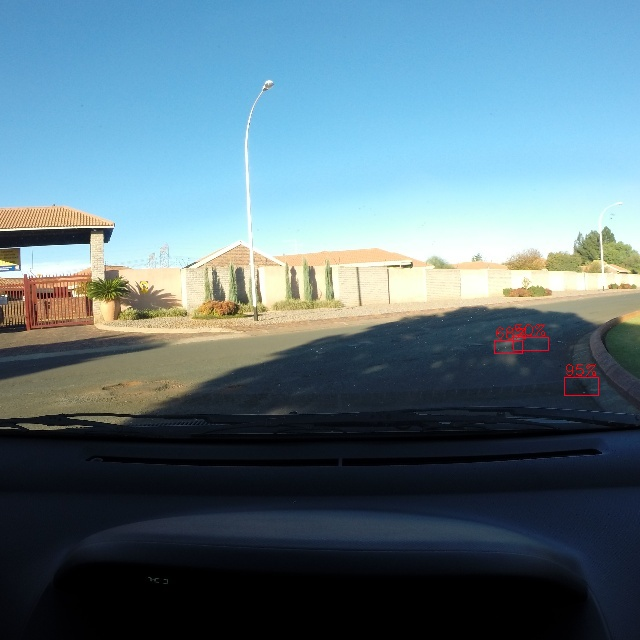
\includegraphics[width=\linewidth]{images/results_a_yolo_v3_tiny_256.jpg}
		\caption{YOLO V3 Tiny tamaño 256x256}
	\end{subfigure}
	\begin{subfigure}[h]{0.45\linewidth}
		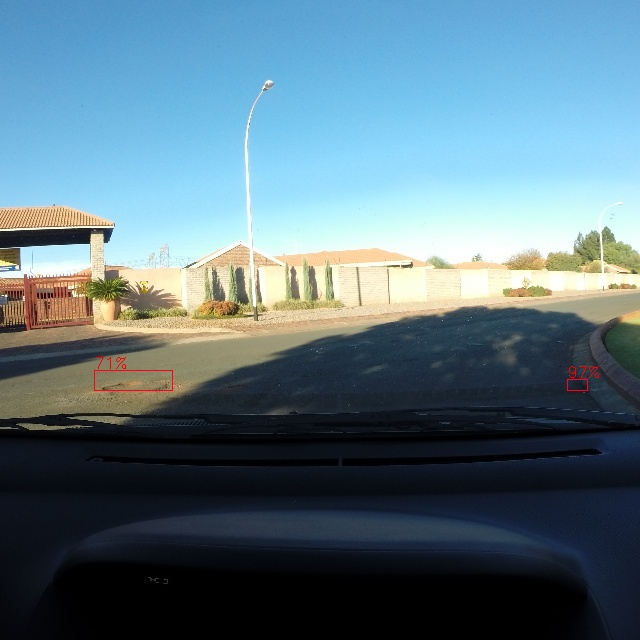
\includegraphics[width=\linewidth]{images/results_a_yolo_v3_tiny_416.jpg}
		\caption{YOLO V3 Tiny tamaño 416x416}
	\end{subfigure}
	\caption{Misma predicción que en la figura \ref{fig:resultsav3}, pero en esta ocasión con modelos YOLO V3 Tiny.}
	\label{fig:resultsav3tiny}
\end{figure}

En la figura \ref{fig:resultsbv3} se muestran más predicciones realizadas por los modelos YOLO V3. En esta ocasión se trata de una imagen en la que hay múltiples baches, de los cuales únicamente se han mantenido 2 y el resto se han descartado. En esta ocasión los 3 modelos detectan baches de forma correcta. El único modelo que detecta los baches esperados es el de tamaño 640x640. Además de detectar los baches detectados, es capaz de detectar uno de los baches que fue descartado por tamaño. Los otros dos modelos de tamaño inferior únicamente detectan uno de los baches esperados, aunque son capaces de detectar también algunos de los baches descartados.

\begin{figure}[H]
	\centering
	\begin{subfigure}[h]{0.45\linewidth}
		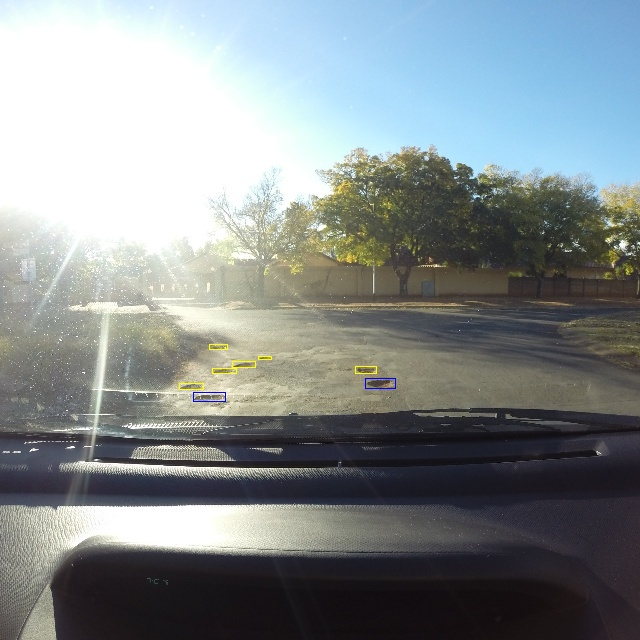
\includegraphics[width=\linewidth]{images/results_b_gt.jpg}
		\caption{Baches a detectar}
	\end{subfigure}
	\begin{subfigure}[h]{0.45\linewidth}
		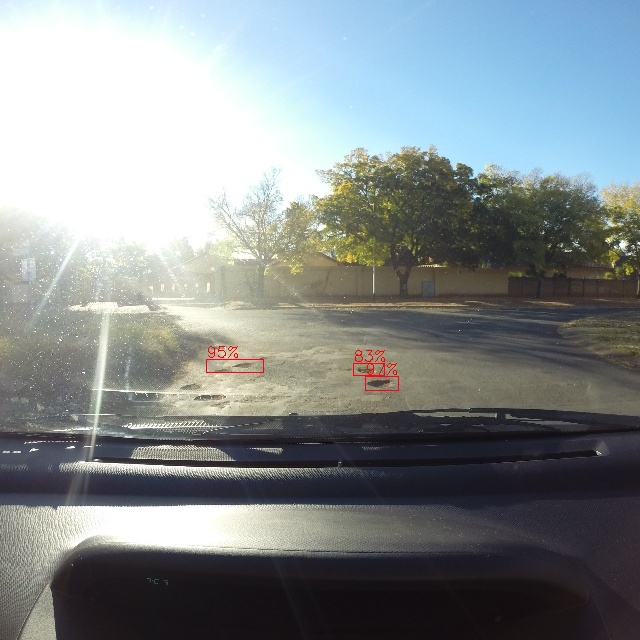
\includegraphics[width=\linewidth]{images/results_b_yolo_v3_256.jpg}
		\caption{YOLO V3 tamaño 256x256}
	\end{subfigure}
	\begin{subfigure}[h]{0.45\linewidth}
		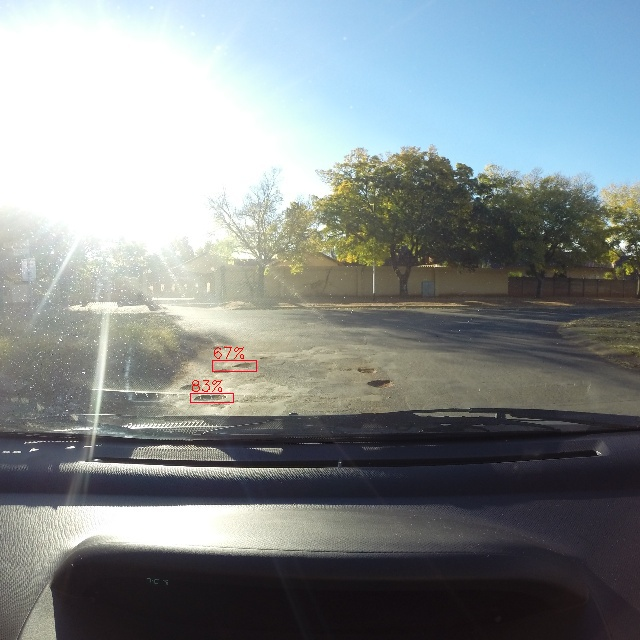
\includegraphics[width=\linewidth]{images/results_b_yolo_v3_416.jpg}
		\caption{YOLO V3 tamaño 416x416}
	\end{subfigure}
	\begin{subfigure}[h]{0.45\linewidth}
		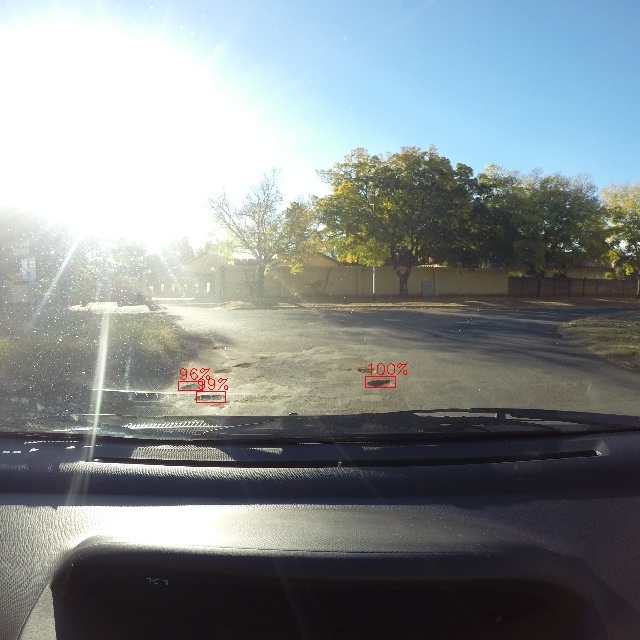
\includegraphics[width=\linewidth]{images/results_b_yolo_v3_640.jpg}
		\caption{YOLO V3 tamaño 640x640}
	\end{subfigure}
	\caption{Ejemplo de predicción con modelos YOLO V3 de distintos tamaños. Arriba a la izquierda, la imagen con los baches a detectar en azul y en amarillo los baches que fueron descartados por el filtro. En el resto de las imágenes se pueden ver las predicciones realizadas en rojo.}
	\label{fig:resultsbv3}
\end{figure}

En la figura \ref{fig:resultsbv3tiny} se muestran las predicciones realizadas por los modelos YOLO V3 Tiny para el segundo ejemplo. En esta ocasión ambos modelos son capaces de detectar baches de forma correcta. Además el modelo de tamaño 416x416 es capaz de identificar los dos baches esperados.

\begin{figure}[H]
	\centering
	\begin{subfigure}[h]{0.45\linewidth}
		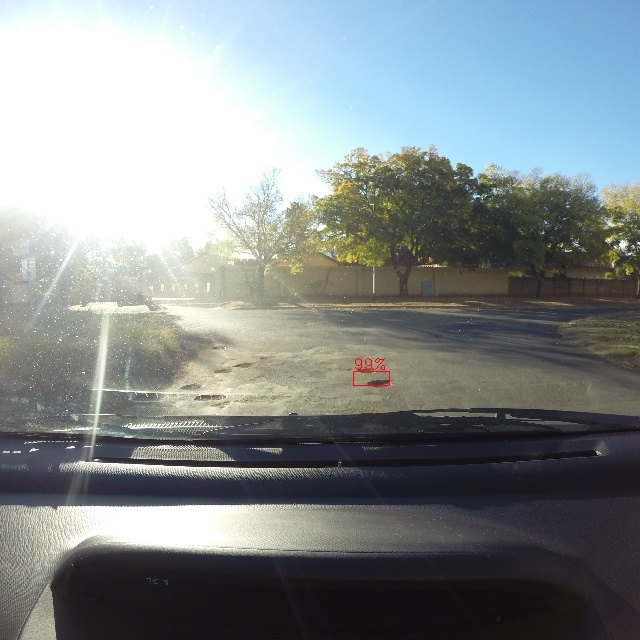
\includegraphics[width=\linewidth]{images/results_b_yolo_v3_tiny_256.jpg}
		\caption{YOLO V3 Tiny tamaño 256x256}
	\end{subfigure}
	\begin{subfigure}[h]{0.45\linewidth}
		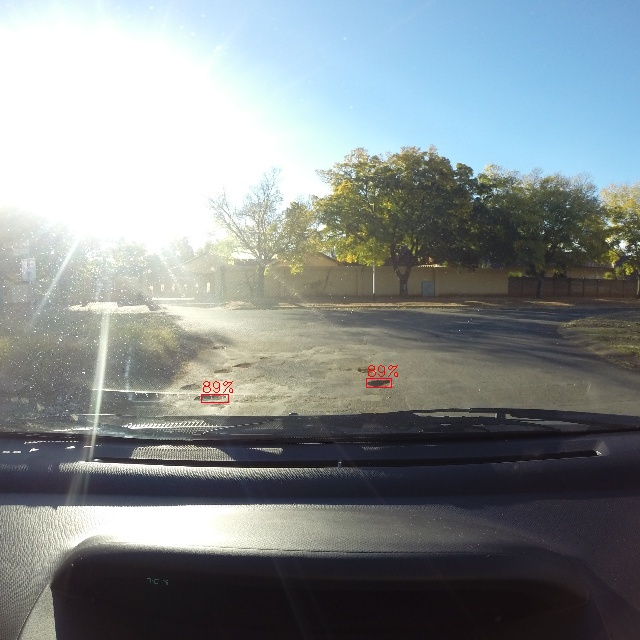
\includegraphics[width=\linewidth]{images/results_b_yolo_v3_tiny_416.jpg}
		\caption{YOLO V3 Tiny tamaño 416x416}
	\end{subfigure}
	\caption{Misma predicción que en la figura \ref{fig:resultsbv3}, pero en esta ocasión con modelos YOLO V3 Tiny.}
	\label{fig:resultsbv3tiny}
\end{figure}

En la figura \ref{fig:resultscv3} se muestra otro ejemplo de predicciones realizadas por los modelos YOLO V3. En esta ocasión también se trata de una imagen en la que hay múltiples baches, de los cuales se ha mantenido un único bache. En esta ocasión uno de los modelos, el de tamaño 416x416, es incapaz de detectar ningún bache. El modelo más pequeño, detecta uno de los baches que ha sido descartado, y además la predicción es mejor al original ya que la región predicha se ajusta más al bache. El modelo más grande ha sido capaz de detectar el bache original y además detecta otro de los baches que fue descartados.

\begin{figure}[H]
	\centering
	\begin{subfigure}[h]{0.45\linewidth}
		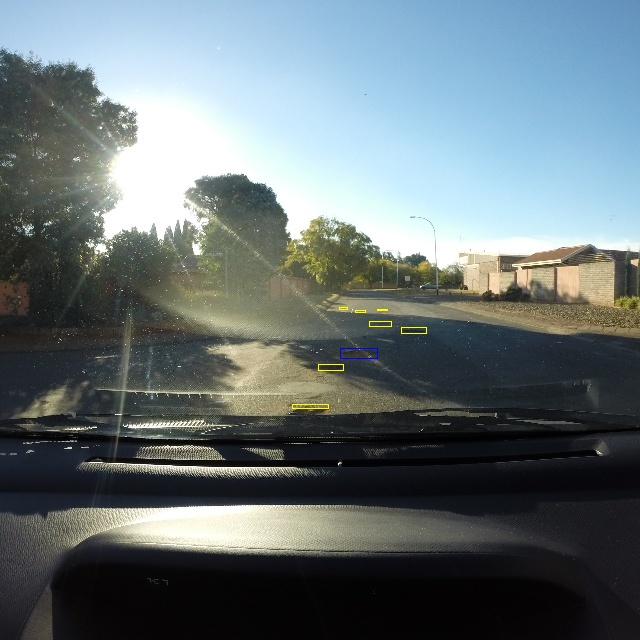
\includegraphics[width=\linewidth]{images/results_c_gt.jpg}
		\caption{Baches a detectar}
	\end{subfigure}
	\begin{subfigure}[h]{0.45\linewidth}
		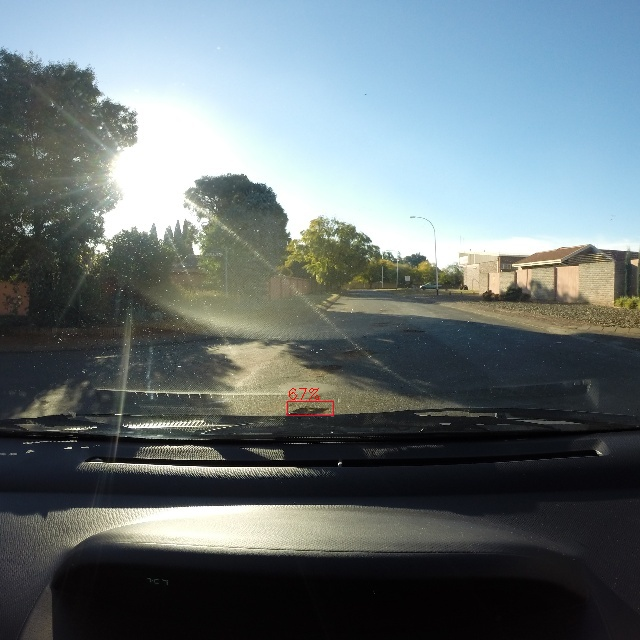
\includegraphics[width=\linewidth]{images/results_c_yolo_v3_256.jpg}
		\caption{YOLO V3 tamaño 256x256}
	\end{subfigure}
	\begin{subfigure}[h]{0.45\linewidth}
		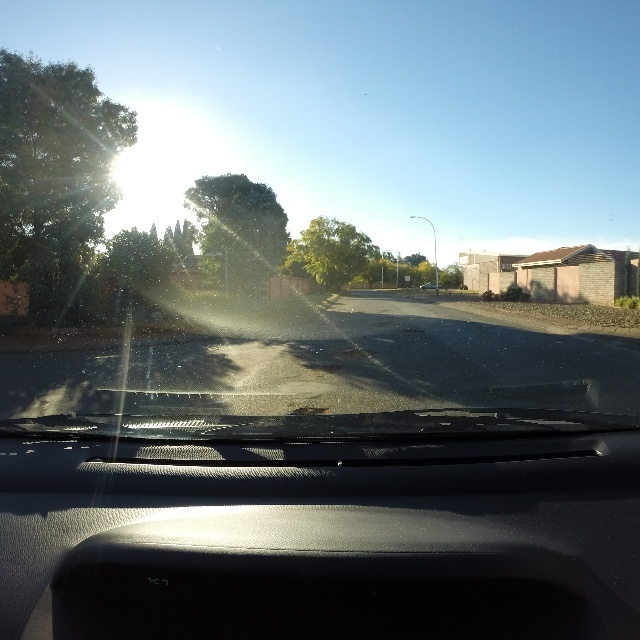
\includegraphics[width=\linewidth]{images/results_c_yolo_v3_416.jpg}
		\caption{YOLO V3 tamaño 416x416}
	\end{subfigure}
	\begin{subfigure}[h]{0.45\linewidth}
		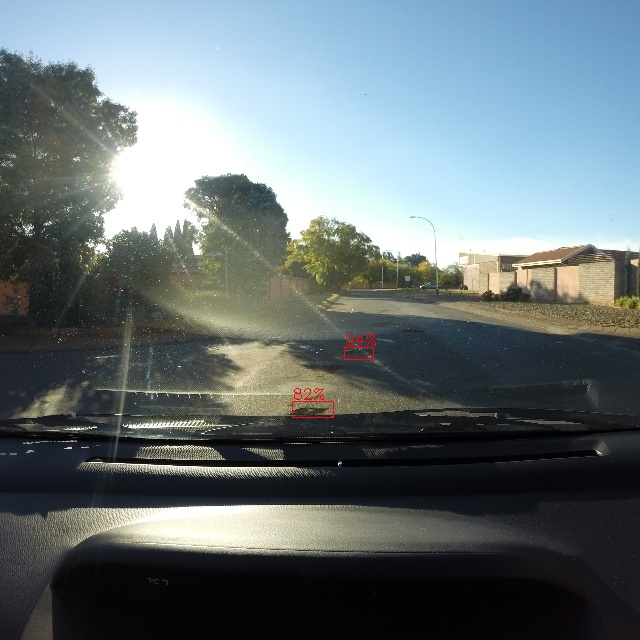
\includegraphics[width=\linewidth]{images/results_c_yolo_v3_640.jpg}
		\caption{YOLO V3 tamaño 640x640}
	\end{subfigure}
	\caption{Ejemplo de predicción con modelos YOLO V3 de distintos tamaños. Arriba a la izquierda, la imagen con los baches a detectar en azul y en amarillo los baches que fueron descartados por el filtro. En el resto de las imágenes se pueden ver las predicciones realizadas en rojo.}
	\label{fig:resultscv3}
\end{figure}

En la figura \ref{fig:resultscv3tiny} se pueden ver las predicciones realizadas por los modelos YOLO V3 Tiny para el ejemplo anterior. Sólo uno de los modelos detecta uno de los baches.

\begin{figure}[H]
	\centering
	\begin{subfigure}[h]{0.45\linewidth}
		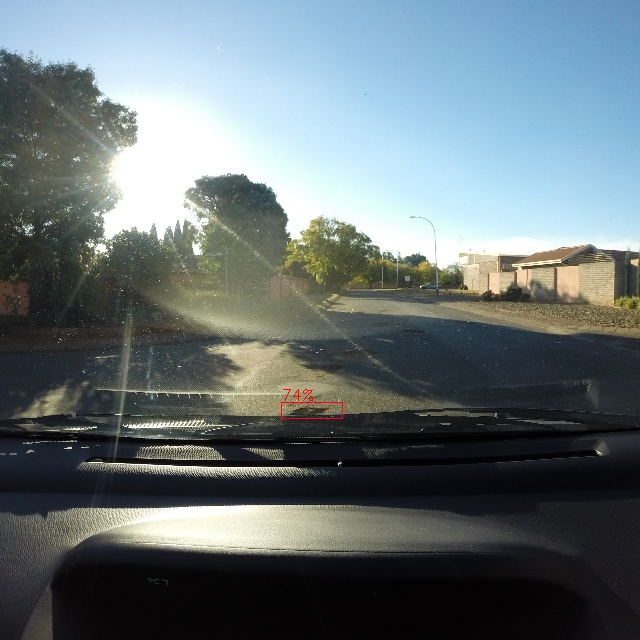
\includegraphics[width=\linewidth]{images/results_c_yolo_v3_tiny_256.jpg}
		\caption{YOLO V3 Tiny tamaño 256x256}
	\end{subfigure}
	\begin{subfigure}[h]{0.45\linewidth}
		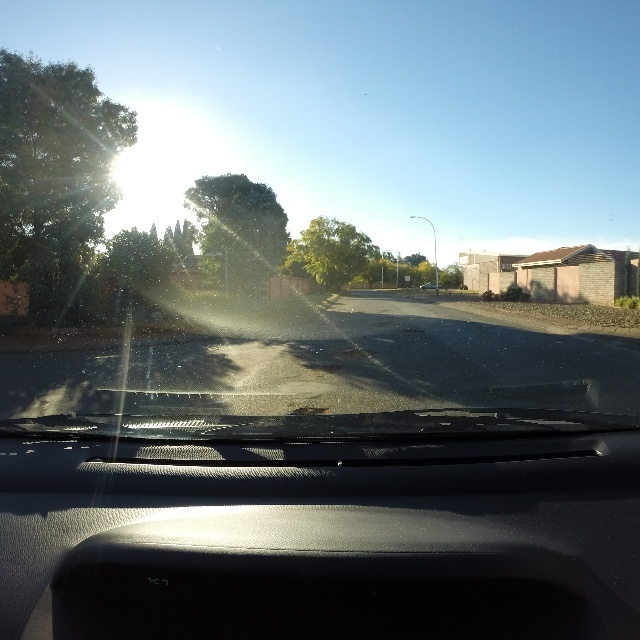
\includegraphics[width=\linewidth]{images/results_c_yolo_v3_tiny_416.jpg}
		\caption{YOLO V3 Tiny tamaño 416x416}
	\end{subfigure}
	\caption{Misma predicción que en la figura \ref{fig:resultscv3}, pero en esta ocasión con modelos YOLO V3 Tiny.}
	\label{fig:resultscv3tiny}
\end{figure}

En la figura \ref{fig:resultsdv3} se muestra un ejemplo más de predicciones realizadas por los modelos YOLO V3. En esta ocasión también se trata de una imagen en la que hay múltiples baches, de los cuales se han mantenido dos. Todos los modelos han sido capaces de detectar los baches originales, aunque no de la misma forma. Uno de los baches originales se encuentra contiguo a otro descartado. Las regiones propuestas por los dos modelos más pequeños para este bache no son muy precisas porque abarcan ambos baches. Esto no ocurre así para el modelo más grande.

\begin{figure}[H]
	\centering
	\begin{subfigure}[h]{0.45\linewidth}
		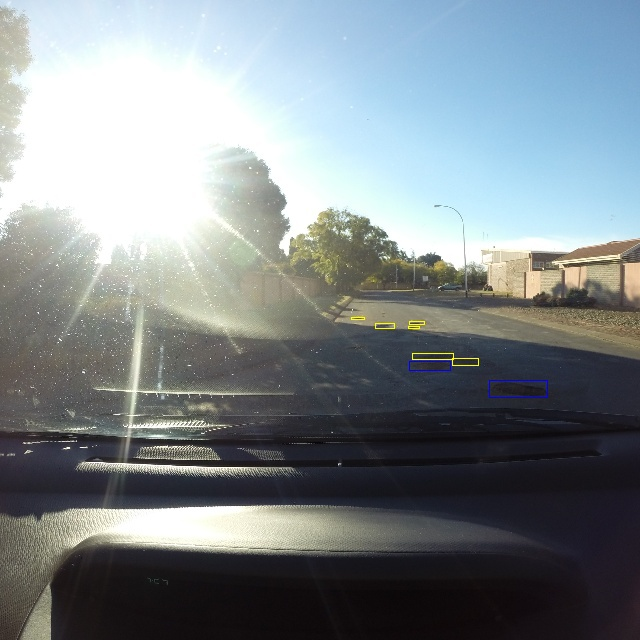
\includegraphics[width=\linewidth]{images/results_d_gt.jpg}
		\caption{Baches a detectar}
	\end{subfigure}
	\begin{subfigure}[h]{0.45\linewidth}
		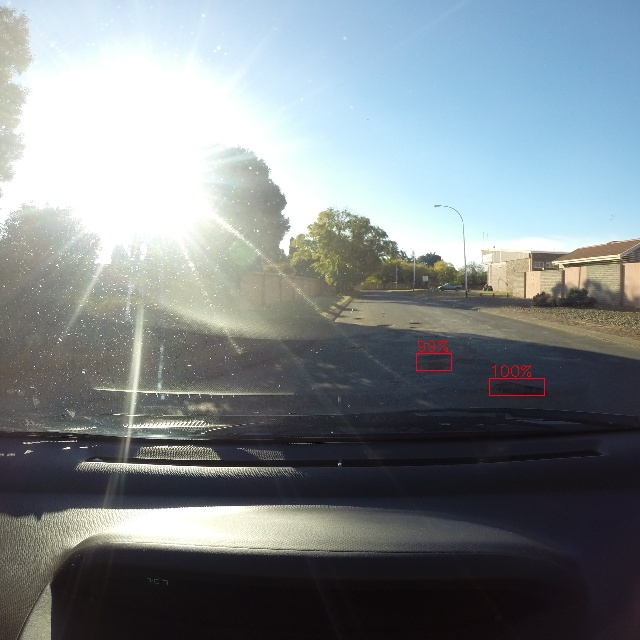
\includegraphics[width=\linewidth]{images/results_d_yolo_v3_256.jpg}
		\caption{YOLO V3 tamaño 256x256}
	\end{subfigure}
	\begin{subfigure}[h]{0.45\linewidth}
		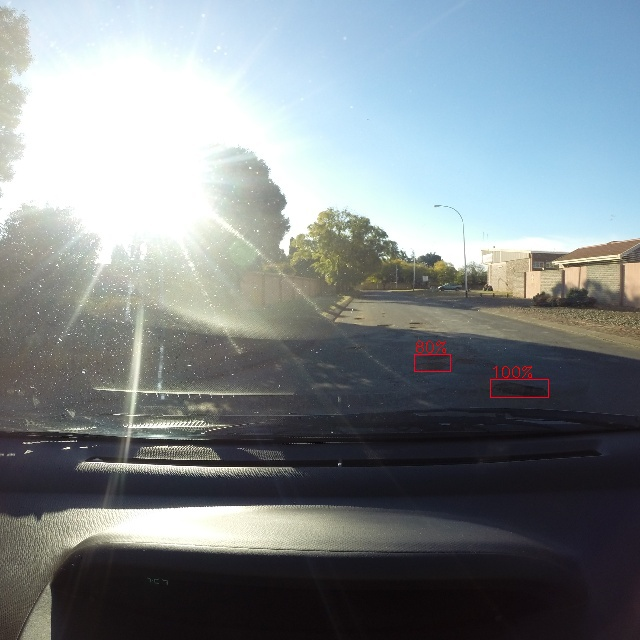
\includegraphics[width=\linewidth]{images/results_d_yolo_v3_416.jpg}
		\caption{YOLO V3 tamaño 416x416}
	\end{subfigure}
	\begin{subfigure}[h]{0.45\linewidth}
		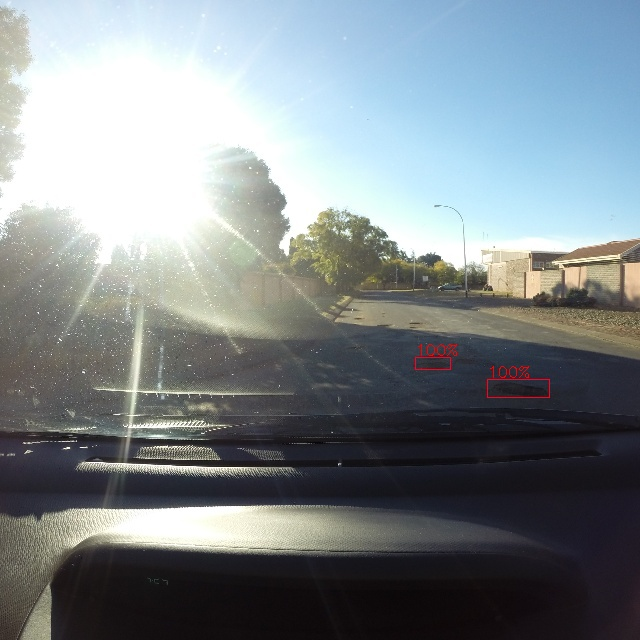
\includegraphics[width=\linewidth]{images/results_d_yolo_v3_640.jpg}
		\caption{YOLO V3 tamaño 640x640}
	\end{subfigure}
	\caption{Ejemplo de predicción con modelos YOLO V3 de distintos tamaños. Arriba a la izquierda, la imagen con los baches a detectar en azul y en amarillo los baches que fueron descartados por el filtro. En el resto de las imágenes se pueden ver las predicciones realizadas en rojo.}
	\label{fig:resultsdv3}
\end{figure}

En la figura \ref{fig:resultsdv3tiny} se pueden ver las predicciones realizadas por los modelos YOLO V3 Tiny para el ejemplo anterior. Ambos modelos detectan los baches, aunque se están haciendo predicciones adicionales que son erróneas.

\begin{figure}[H]
	\centering
	\begin{subfigure}[h]{0.45\linewidth}
		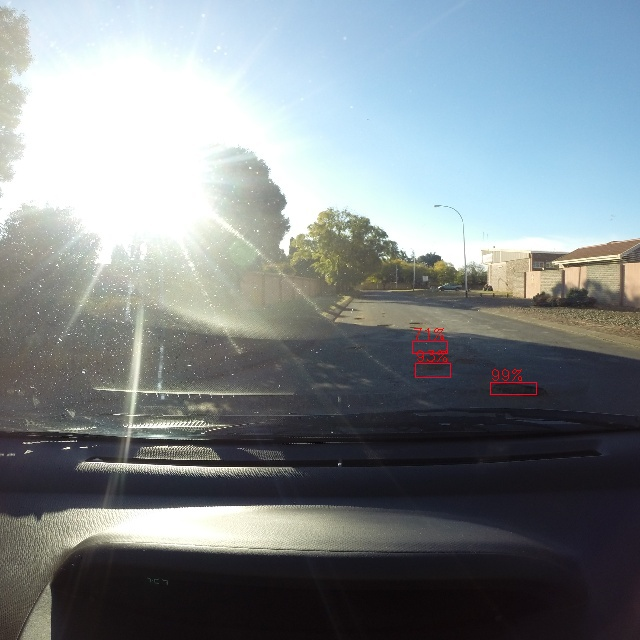
\includegraphics[width=\linewidth]{images/results_d_yolo_v3_tiny_256.jpg}
		\caption{YOLO V3 Tiny tamaño 256x256}
	\end{subfigure}
	\begin{subfigure}[h]{0.45\linewidth}
		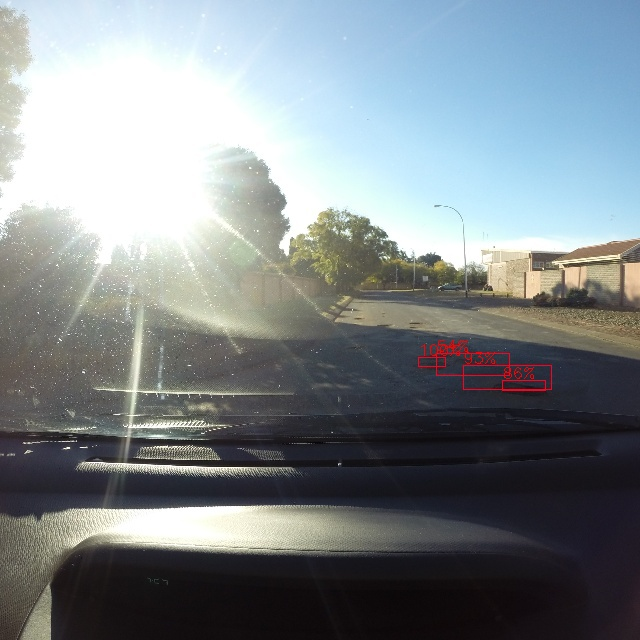
\includegraphics[width=\linewidth]{images/results_d_yolo_v3_tiny_416.jpg}
		\caption{YOLO V3 Tiny tamaño 416x416}
	\end{subfigure}
	\caption{Misma predicción que en la figura \ref{fig:resultsdv3}, pero en esta ocasión con modelos YOLO V3 Tiny.}
	\label{fig:resultsdv3tiny}
\end{figure}

En la figura \ref{fig:resultsev3} se muestra un ejemplo más de predicciones realizadas por los modelos YOLO V3. En esta ocasión también se trata de una imagen en la que hay múltiples baches, de los cuales se mantiene uno. Este ejemplo es un poco diferente a los anteriores porque este no es un caso evidente para el ojo humano, aún así, todos los modelos han sido capaces de detectar el bache original.

\begin{figure}[H]
	\centering
	\begin{subfigure}[h]{0.45\linewidth}
		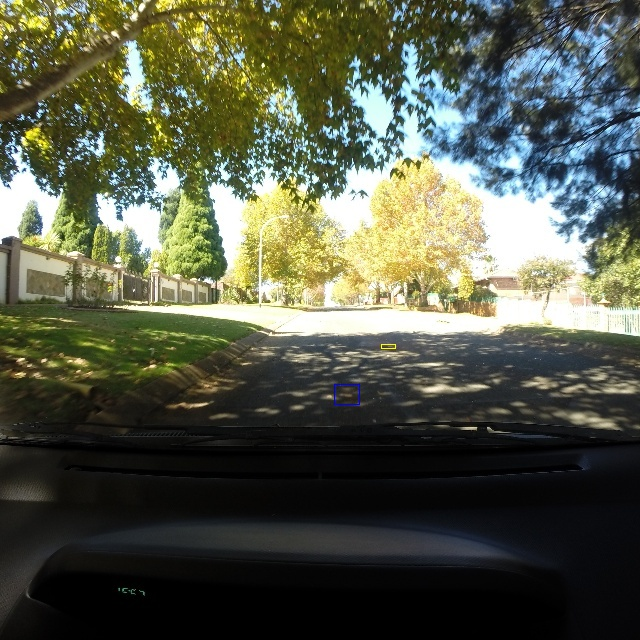
\includegraphics[width=\linewidth]{images/results_e_gt.jpg}
		\caption{Baches a detectar}
	\end{subfigure}
	\begin{subfigure}[h]{0.45\linewidth}
		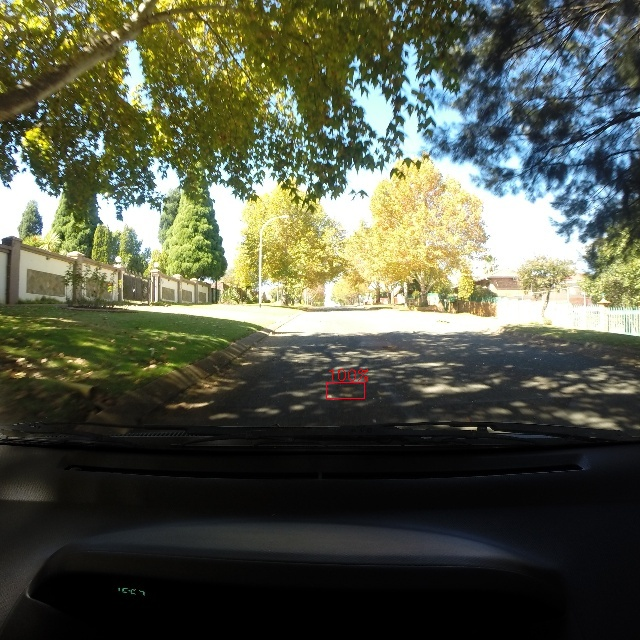
\includegraphics[width=\linewidth]{images/results_e_yolo_v3_256.jpg}
		\caption{YOLO V3 tamaño 256x256}
	\end{subfigure}
	\begin{subfigure}[h]{0.45\linewidth}
		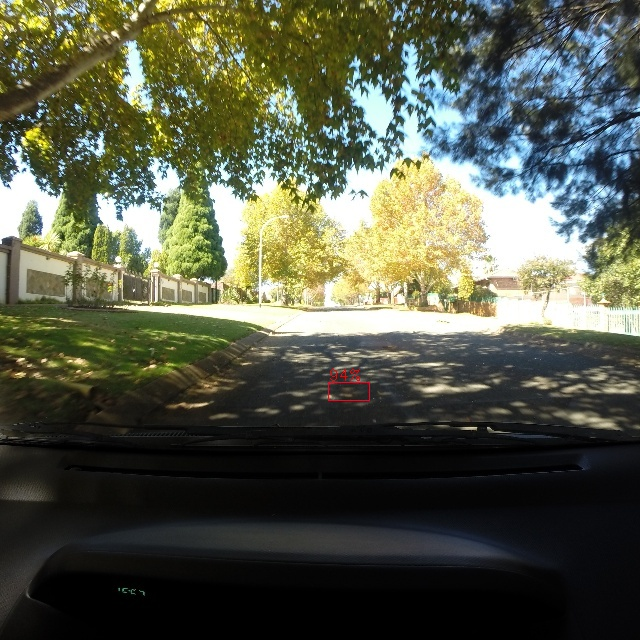
\includegraphics[width=\linewidth]{images/results_e_yolo_v3_416.jpg}
		\caption{YOLO V3 tamaño 416x416}
	\end{subfigure}
	\begin{subfigure}[h]{0.45\linewidth}
		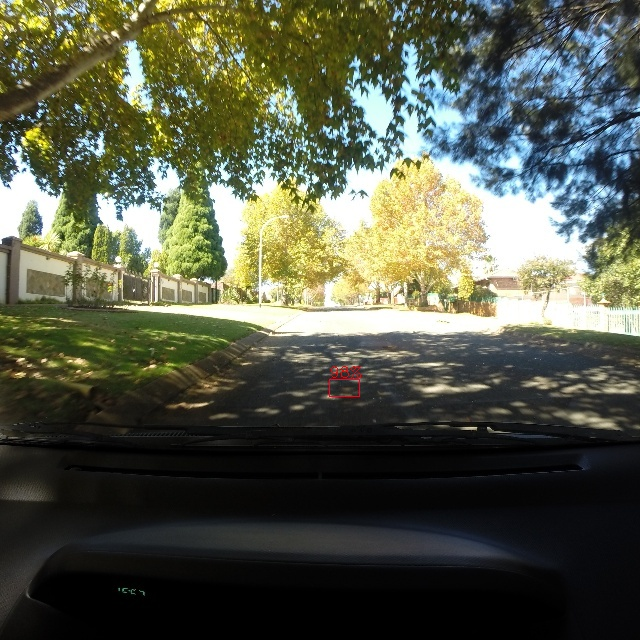
\includegraphics[width=\linewidth]{images/results_e_yolo_v3_640.jpg}
		\caption{YOLO V3 tamaño 640x640}
	\end{subfigure}
	\caption{Ejemplo de predicción con modelos YOLO V3 de distintos tamaños. Arriba a la izquierda, la imagen con los baches a detectar en azul y en amarillo los baches que fueron descartados por el filtro. En el resto de las imágenes se pueden ver las predicciones realizadas en rojo.}
	\label{fig:resultsev3}
\end{figure}

En la figura \ref{fig:resultsev3tiny} se pueden ver las predicciones realizadas por los modelos YOLO V3 Tiny para el ejemplo anterior. Sólo uno de los modelos es capaz de hacer una predicción, y además errónea.

\begin{figure}[H]
	\centering
	\begin{subfigure}[h]{0.45\linewidth}
		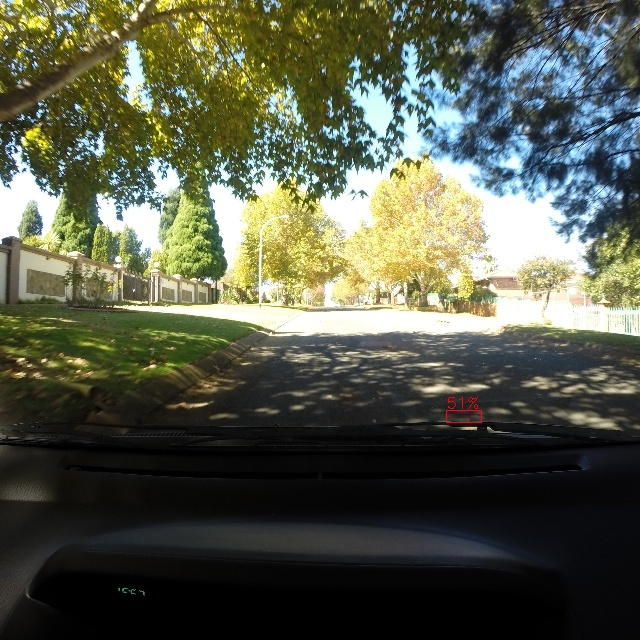
\includegraphics[width=\linewidth]{images/results_e_yolo_v3_tiny_256.jpg}
		\caption{YOLO V3 Tiny tamaño 256x256}
	\end{subfigure}
	\begin{subfigure}[h]{0.45\linewidth}
		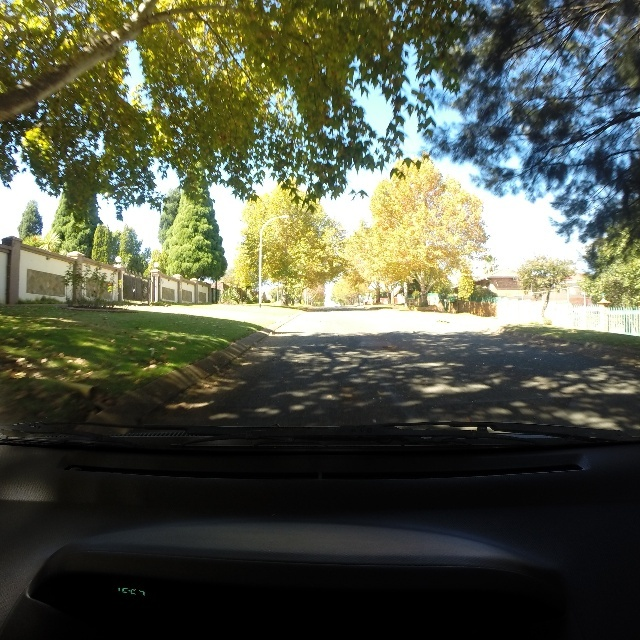
\includegraphics[width=\linewidth]{images/results_e_yolo_v3_tiny_416.jpg}
		\caption{YOLO V3 Tiny tamaño 416x416}
	\end{subfigure}
	\caption{Misma predicción que en la figura \ref{fig:resultsev3}, pero en esta ocasión con modelos YOLO V3 Tiny.}
	\label{fig:resultsev3tiny}
\end{figure}

En la figura \ref{fig:resultsfv3} se muestra un último ejemplo de predicciones realizadas por los modelos YOLO V3. En esta ocasión se trata de una imagen en la que hay un único bache. Todos los modelos tienen un comportamiento errático, además de detectar el bache, se han visto afectados por las hojas en el asfalto realizando predicciones erróneas.

\begin{figure}[H]
	\centering
	\begin{subfigure}[h]{0.45\linewidth}
		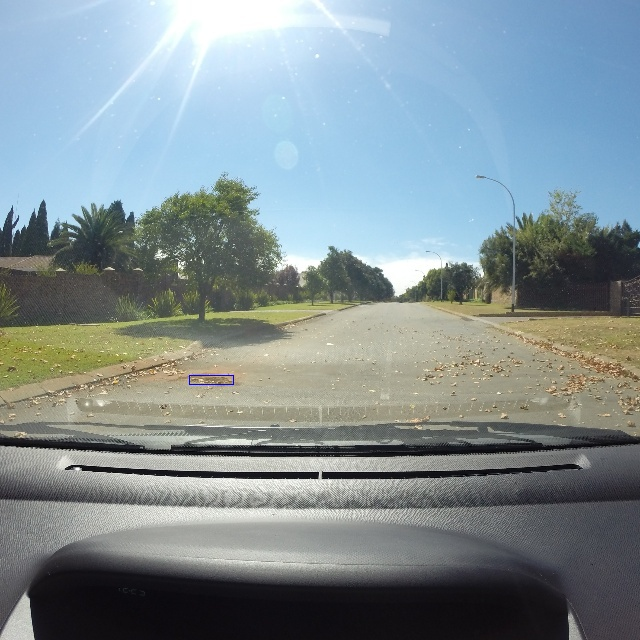
\includegraphics[width=\linewidth]{images/results_f_gt.jpg}
		\caption{Baches a detectar}
	\end{subfigure}
	\begin{subfigure}[h]{0.45\linewidth}
		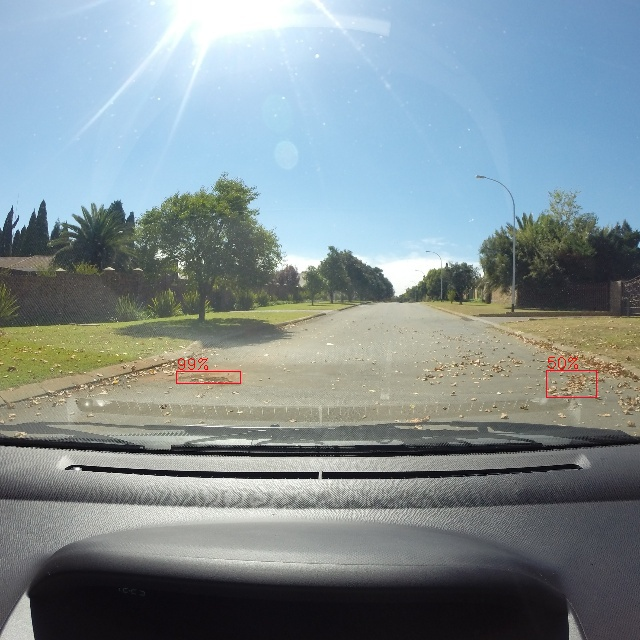
\includegraphics[width=\linewidth]{images/results_f_yolo_v3_256.jpg}
		\caption{YOLO V3 tamaño 256x256}
	\end{subfigure}
	\begin{subfigure}[h]{0.45\linewidth}
		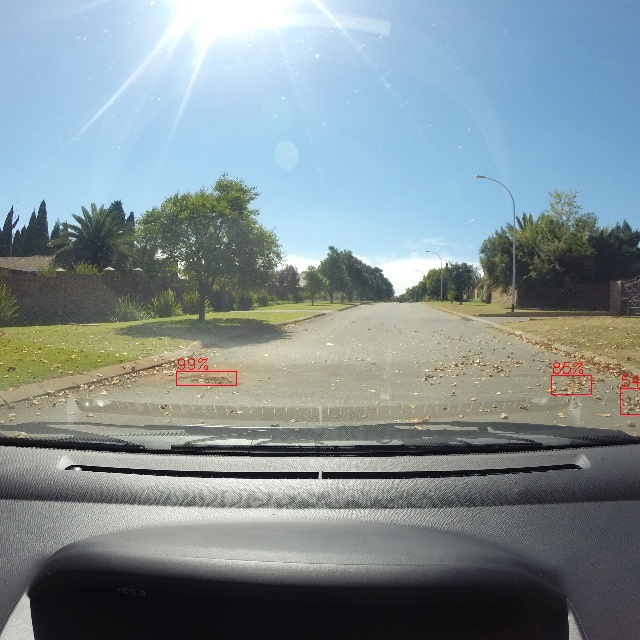
\includegraphics[width=\linewidth]{images/results_f_yolo_v3_416.jpg}
		\caption{YOLO V3 tamaño 416x416}
	\end{subfigure}
	\begin{subfigure}[h]{0.45\linewidth}
		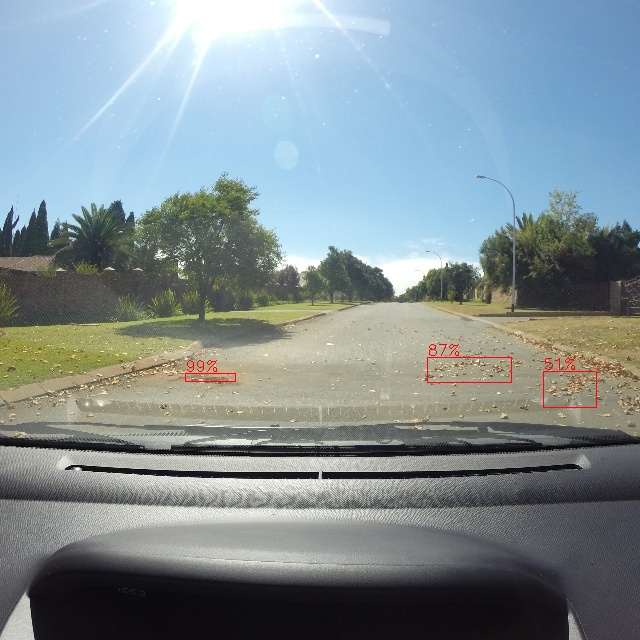
\includegraphics[width=\linewidth]{images/results_f_yolo_v3_640.jpg}
		\caption{YOLO V3 tamaño 640x640}
	\end{subfigure}
	\caption{Ejemplo de predicción con modelos YOLO V3 de distintos tamaños. Arriba a la izquierda, la imagen con los baches a detectar en azul y en amarillo los baches que fueron descartados por el filtro. En el resto de las imágenes se pueden ver las predicciones realizadas en rojo.}
	\label{fig:resultsfv3}
\end{figure}

En la figura \ref{fig:resultsfv3tiny} se pueden ver las predicciones realizadas por los modelos YOLO V3 Tiny para el ejemplo anterior. Estos modelos se han visto afectados de la misma manera por las hojas en el asfalto.

\begin{figure}[H]
	\centering
	\begin{subfigure}[h]{0.45\linewidth}
		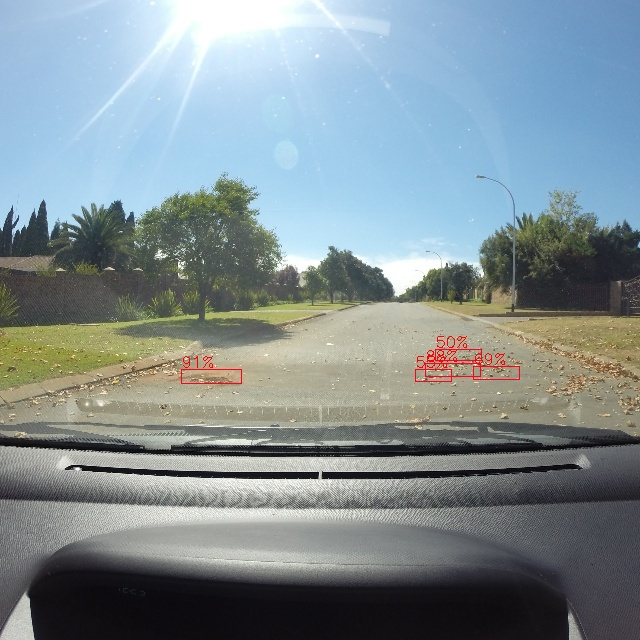
\includegraphics[width=\linewidth]{images/results_f_yolo_v3_tiny_256.jpg}
		\caption{YOLO V3 Tiny tamaño 256x256}
	\end{subfigure}
	\begin{subfigure}[h]{0.45\linewidth}
		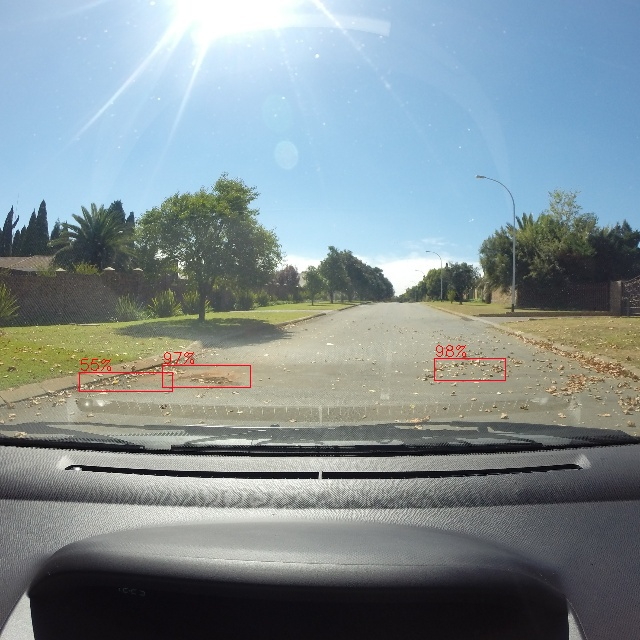
\includegraphics[width=\linewidth]{images/results_f_yolo_v3_tiny_416.jpg}
		\caption{YOLO V3 Tiny tamaño 416x416}
	\end{subfigure}
	\caption{Misma predicción que en la figura \ref{fig:resultsfv3}, pero en esta ocasión con modelos YOLO V3 Tiny.}
	\label{fig:resultsfv3tiny}
\end{figure}